\documentclass{article}

\usepackage{lipsum}
\usepackage{amsfonts}
\usepackage{amsmath}
\usepackage{amsthm}
\usepackage{graphicx}
\graphicspath{{figures/12_23_21_learning_aggregates/}}
\usepackage{epstopdf}
\ifpdf%
\DeclareGraphicsExtensions{.eps,.pdf,.png,.jpg}
\else
\DeclareGraphicsExtensions{.eps}
\fi
\usepackage{amsopn}
\DeclareMathOperator{\diag}{diag}
\usepackage{booktabs}
\usepackage{bbm}
\usepackage{bm}
\usepackage{caption}
\usepackage{subcaption}
\usepackage[utf8]{inputenc}
\usepackage[T1]{fontenc}
\usepackage[margin=1in]{geometry}
\usepackage{hyperref}
\usepackage{algorithm}
\usepackage{algpseudocode}

\newcommand{\norm}[1]{\left\lVert#1\right\rVert}
\newcommand{\normtwo}[1]{\left\lVert#1\right\rVert_2}
\newcommand{\abs}[1]{\left\lvert#1\right\rvert}
\newcommand{\mat}[1]{\bm{{#1}}}
\renewcommand{\vec}[1]{\bm{{#1}}}
\newcommand{\lequiv}{\Leftrightarrow}
\newcommand{\bigO}[1]{\mathcal{O}\!\left(#1\right)}
\newcommand{\ceil}[1]{\left\lceil #1 \right\rceil}
\newcommand{\floor}[1]{\left\lfloor #1 \right\rfloor}
\newcommand{\sfrac}[2]{#1/#2}
\newcommand{\hquad}{\enskip}
\newcommand{\expected}[1]{\mathbb{E}\left[#1\right]}
\newcommand{\mspan}[1]{\text{span}\left( #1 \right)}
\newcommand{\prob}[1]{P\left(#1\right)}
\newcommand{\probt}[1]{P\left( \text{#1} \right)}
\newcommand{\condprob}[2]{P\left(#1 \:|\: #2\right)}
\newcommand{\condprobt}[2]{P\left(\text{#1} \:|\: \text{#2}\right)}
\newcommand{\bayes}[2]{\frac{\condprob{#2}{#1}\prob{#1}}{\prob{#2}}}
\newcommand{\bayesx}[3]{\frac{\condprob{#2}{#1}\prob{#1}}{\condprob{#2}{#1}\prob{#1} + \condprob{#2}{#3}\prob{#3}}}
\newcommand{\sech}{\text{sech}}
\newcommand*{\vertbar}{\rule[-1ex]{0.5pt}{2.5ex}}
\newcommand*{\horzbar}{\rule[.5ex]{2.5ex}{0.5pt}}
\newcommand{\vect}[2]{\underline{{#1}}_{{#2}}}
\newcommand{\basisp}[1]{\underline{{p}}_{{#1}}}
\newcommand{\basisq}[1]{\underline{{q}}_{{#1}}}
\newcommand{\coeff}[1]{\underline{{a}}_{{#1}}}
\newcommand{\bestfit}{\underline{\bar{x}}}
\newcommand{\grad}{\nabla}
\newcommand{\laplace}{\Delta}
\newcommand{\setbar}{\:\middle|\:}
\renewcommand{\div}{\grad \cdot}
\renewcommand{\Re}{\text{Re}}

\begin{document}
\section{Background}
Here, we are attempting to train an ML agent to output both aggregates and interpolation for an AMG solver given some matrix $\mat{A}$.  We will explore how well such an agent can learn to generalize on an \textit{isotropic diffusion problem}, by generating:
\begin{enumerate}
\item A training set of 300 structured grids and 700 unstructured grids.
\item A testing set of 75 structured grids and 175 unstructured grids.
\end{enumerate}
Each of these grid meshes are fairly small, randomly containing somewhere between $25$ and $225$ points.  In the unstructured case, random points are generated in $\left[0,1\right]^2$, then meshed with a Delaunay triangulation.  However, due to computational costs, only $1/8$ of the training set and $1/4$ of the testing set are loaded during GA training.

\section{Generating Aggregates and Interpolation}
To compute the aggregates and final interpolation operator, two individual networks are trained concurrently to perform each action, which we will label $\Theta_{\text{Agg}}$ and $\Theta_{\text{Interp}}$, both taking some weighted graph and returning a new graph with same connectivity, but different weight values.  The algorithm for finding the aggregates and interpolation is roughly sketched below:
\begin{enumerate}
\item Let $\mat{A} \in \mathbb{R}^{n \times n}$ be the system we are trying to solve and $\alpha \in \left(0, 1\right]$ be some parameter that determines the ratio of aggregates to vertices, i.e. we will be roughly coarsening the graph by $1/\alpha$.  Define $k := \ceil{\alpha n}$, the number of aggregates we will be outputting.
\item Convolve the graph of $\mat{A}$ with $\Theta_{\text{Agg}}$ to obtain a new set of node values and edge values.  We will use the node values as a \textit{scoring} and the edge values as path weights.  Define the aggregate centers as the indices of the largest $k$ node scores.  Then, run Bellman-Ford on the graph with these aggregate centers and new edge weights to obtain a tentative aggregation operator, $\text{Agg}$.
\item Now, again convolve the graph of $\mat{A}$ but with $\Theta_{\text{Interp}}$ (with aggregate information) to obtain the aggregate smoother $\mat{\hat{P}}$.  Form $\mat{P} := \mat{\hat{P}}\text{Agg}$.
\end{enumerate}

\section{Genetic Training}
Training of both networks is done at the same time with PyGAD\cite{gad2021pygad}, a genetic algorithm that can be used to train networks without any gradient information.  A basic overview of the training algorithm is that the method is seeded with some number of randomly generated networks. A subset of the best performing (most fit) networks are selected and ``bred'' with one another (crossing weights/traits) and ``mutations'' inserted (random perturbations to weights) to create another population of networks.  This is then repeated for many ``generations'' until a set of hopefully trained networks is obtained, from which we can pick the best fit as our final network.

\section{Results}
The loss values for both the training and testing datasets are displayed in figure \ref{fig:loss}.  The loss is the average convergence for the dataset: in both cases the average convergence for the ML method outperforms the average baseline loss after approximately 30 or so generations.
\begin{figure}[h]
  \centering
  \begin{subfigure}[t]{0.49\textwidth}
    \centering
    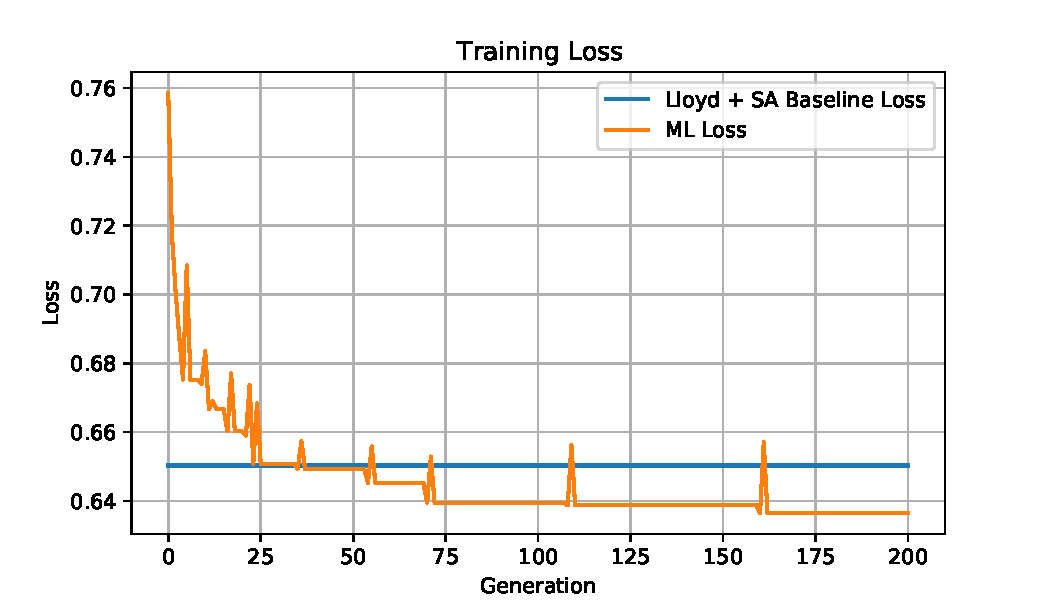
\includegraphics[width=\textwidth]{train_loss.pdf}
    \caption{Training loss}
  \end{subfigure}
  \hfill
  \begin{subfigure}[t]{0.49\textwidth}
    \centering
    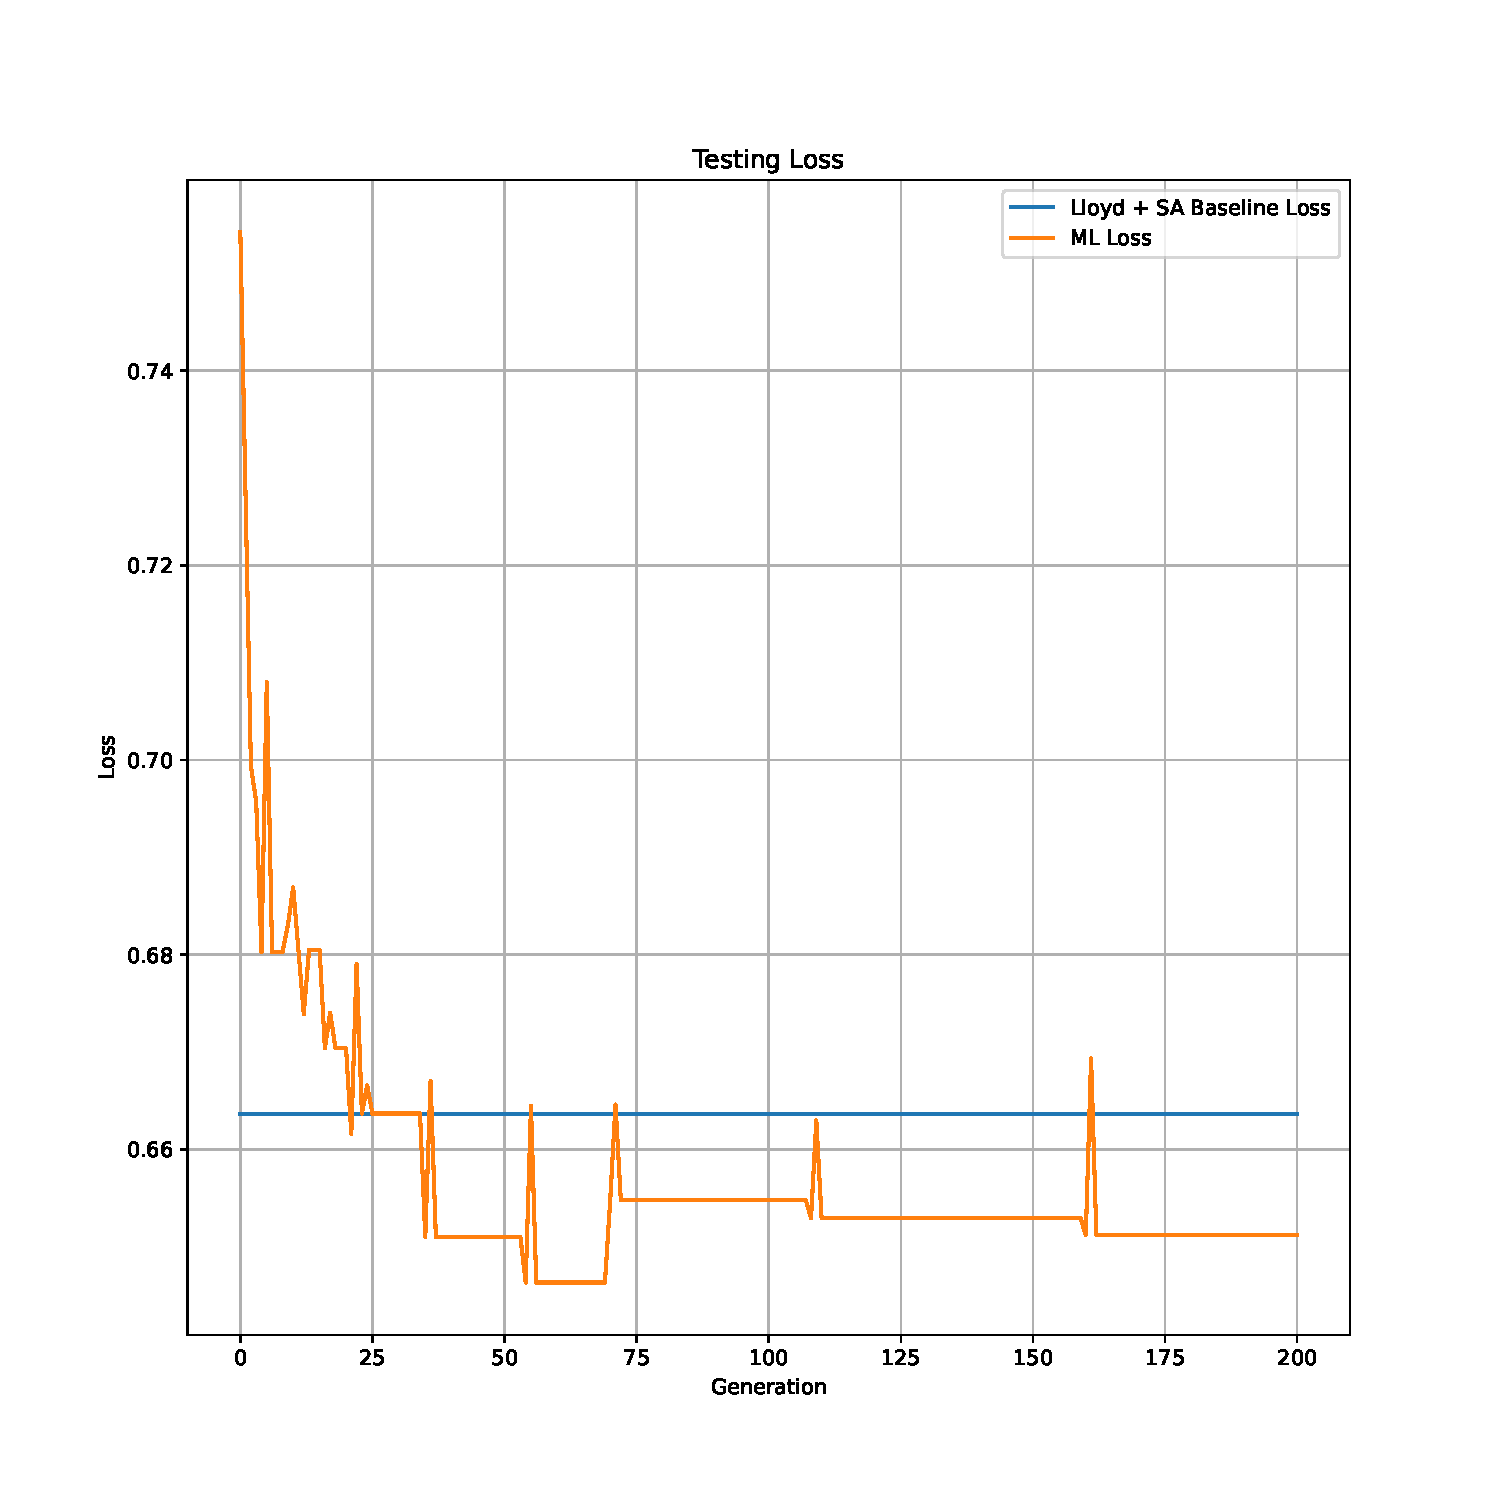
\includegraphics[width=\textwidth]{test_loss.pdf}
    \caption{Testing loss}
  \end{subfigure}
  \caption{Loss plots per generation for training and testing datasets, respectively.}
  \label{fig:loss}
\end{figure}

Convergence for all generated grids is displayed in Figure \ref{fig:conv}, with baseline convergence along the $x$-axis and ML convergence along the $y$-axis.  The figure should be read by comparing points to their position relative to the diagonal.  Samples where the ML and baseline method are equal will result in a position directly on the diagonal line, while those where the ML method is more convergent will give a position below the diagonal.  A better baseline convergence will place samples above the diagonal line.
\begin{figure}[h]
  \centering
  \begin{subfigure}[t]{0.49\textwidth}
    \centering
    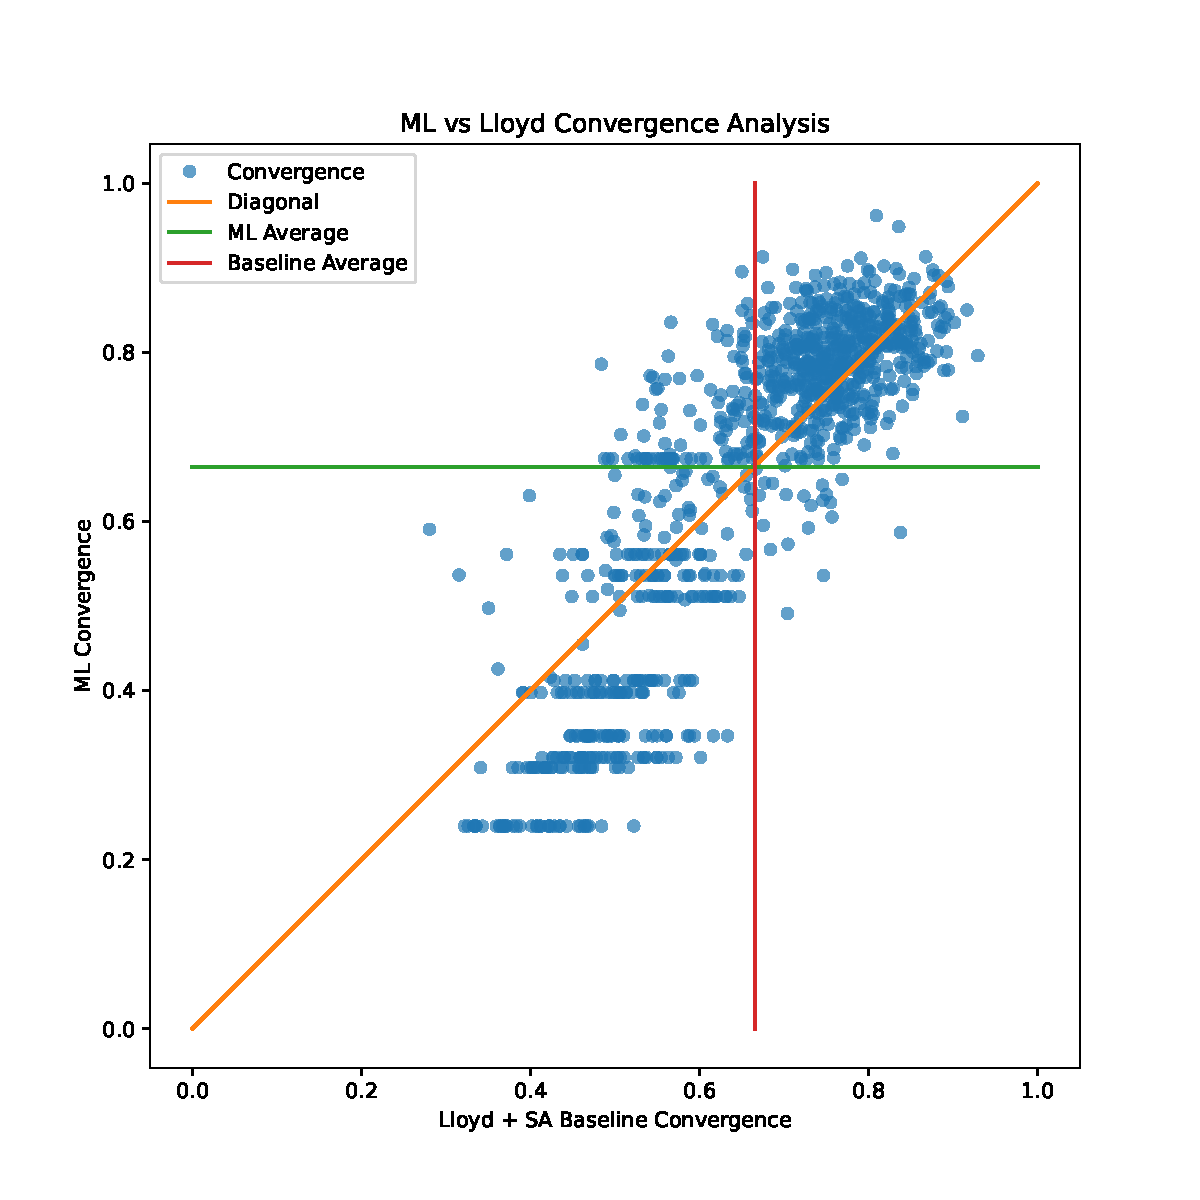
\includegraphics[width=\textwidth]{train_convergence.pdf}
    \caption{Training convergence}
  \end{subfigure}
  \begin{subfigure}[t]{0.49\textwidth}
    \centering
    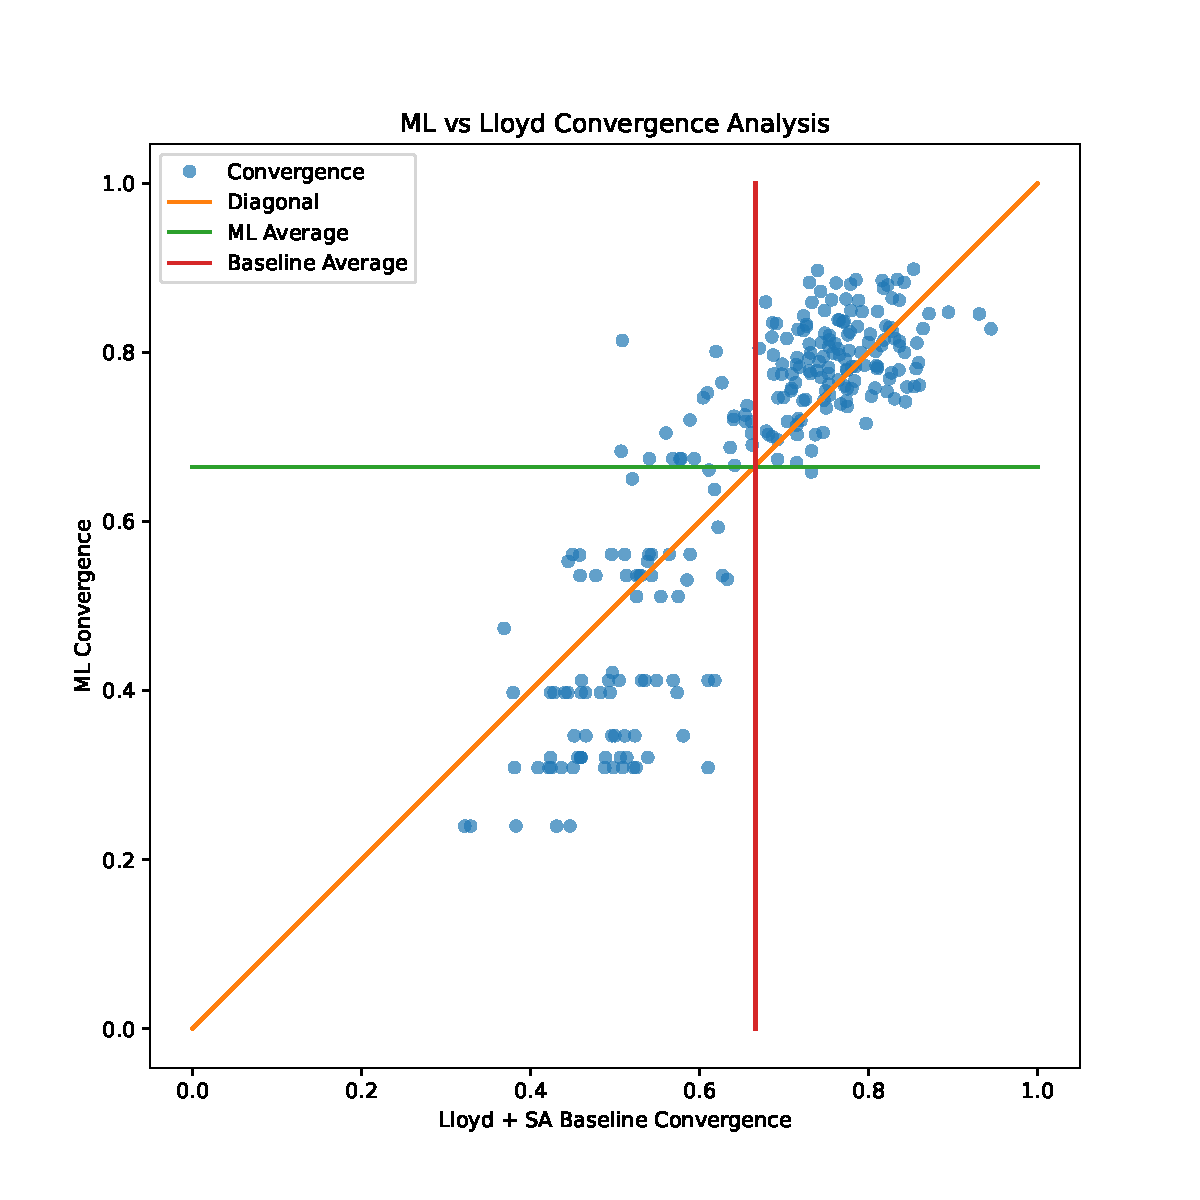
\includegraphics[width=\textwidth]{test_convergence.pdf}
    \caption{Testing convergence}
  \end{subfigure}
  \caption{Convergence data for the ML AMG method vs a baseline Lloyd and Jacobi SA method.  Values below the diagonal indicate a better convergence for the ML.}
  \label{fig:conv}
\end{figure}

Aggregate and interpolation data for a few structured grids are shown in Figures \ref{fig:grid12}, \ref{fig:grid14}, \ref{fig:grid15}.  Notice the lousy aggregates for the $15\times 15$ case; in theory the ML method should have seen such a grid during training, yet it is unable to generalize.
\begin{figure}[h]
  \centering
  \begin{subfigure}[t]{0.49\textwidth}
    \centering
    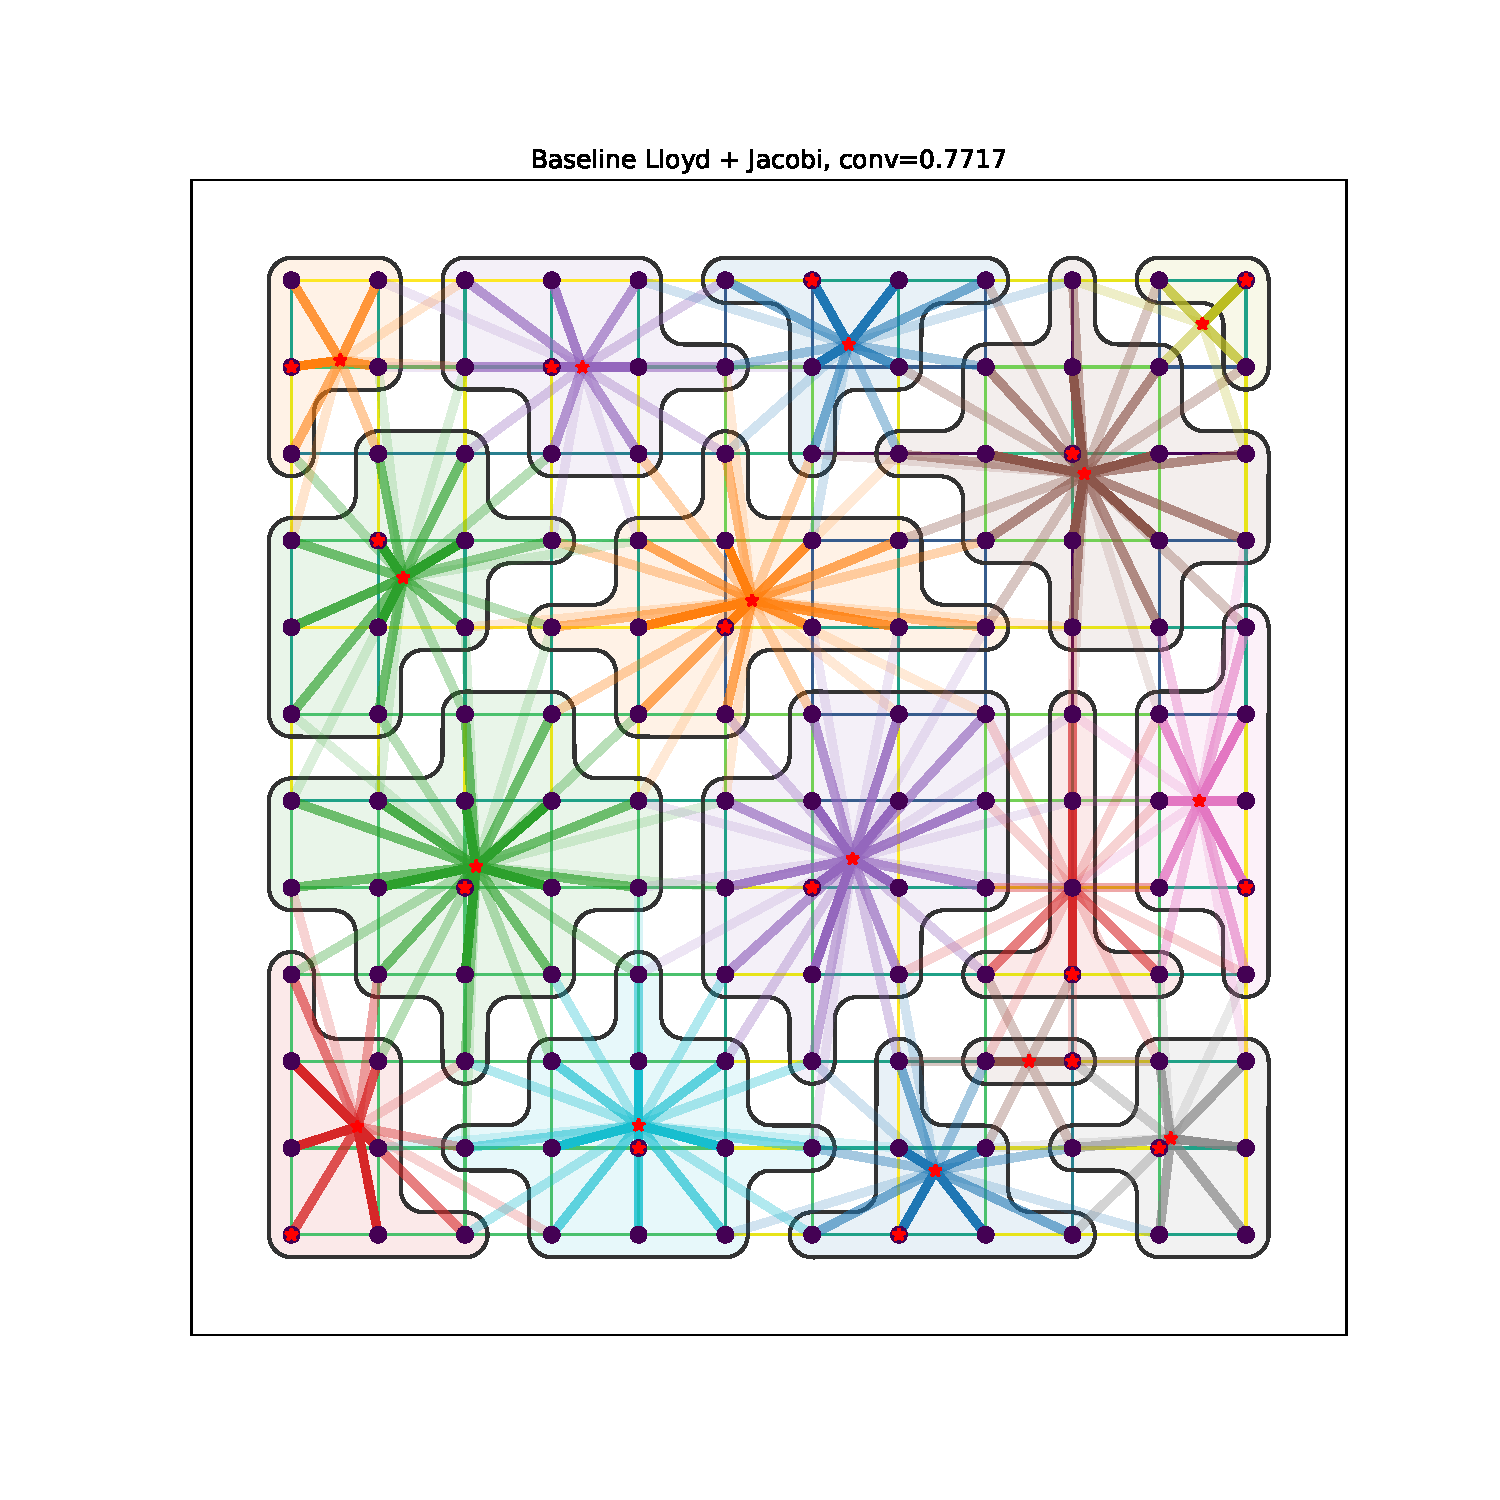
\includegraphics[width=\textwidth]{grid_12_lloyd.pdf}
    \caption{Lloyd + Jacobi}
  \end{subfigure}
  \begin{subfigure}[t]{0.49\textwidth}
    \centering
    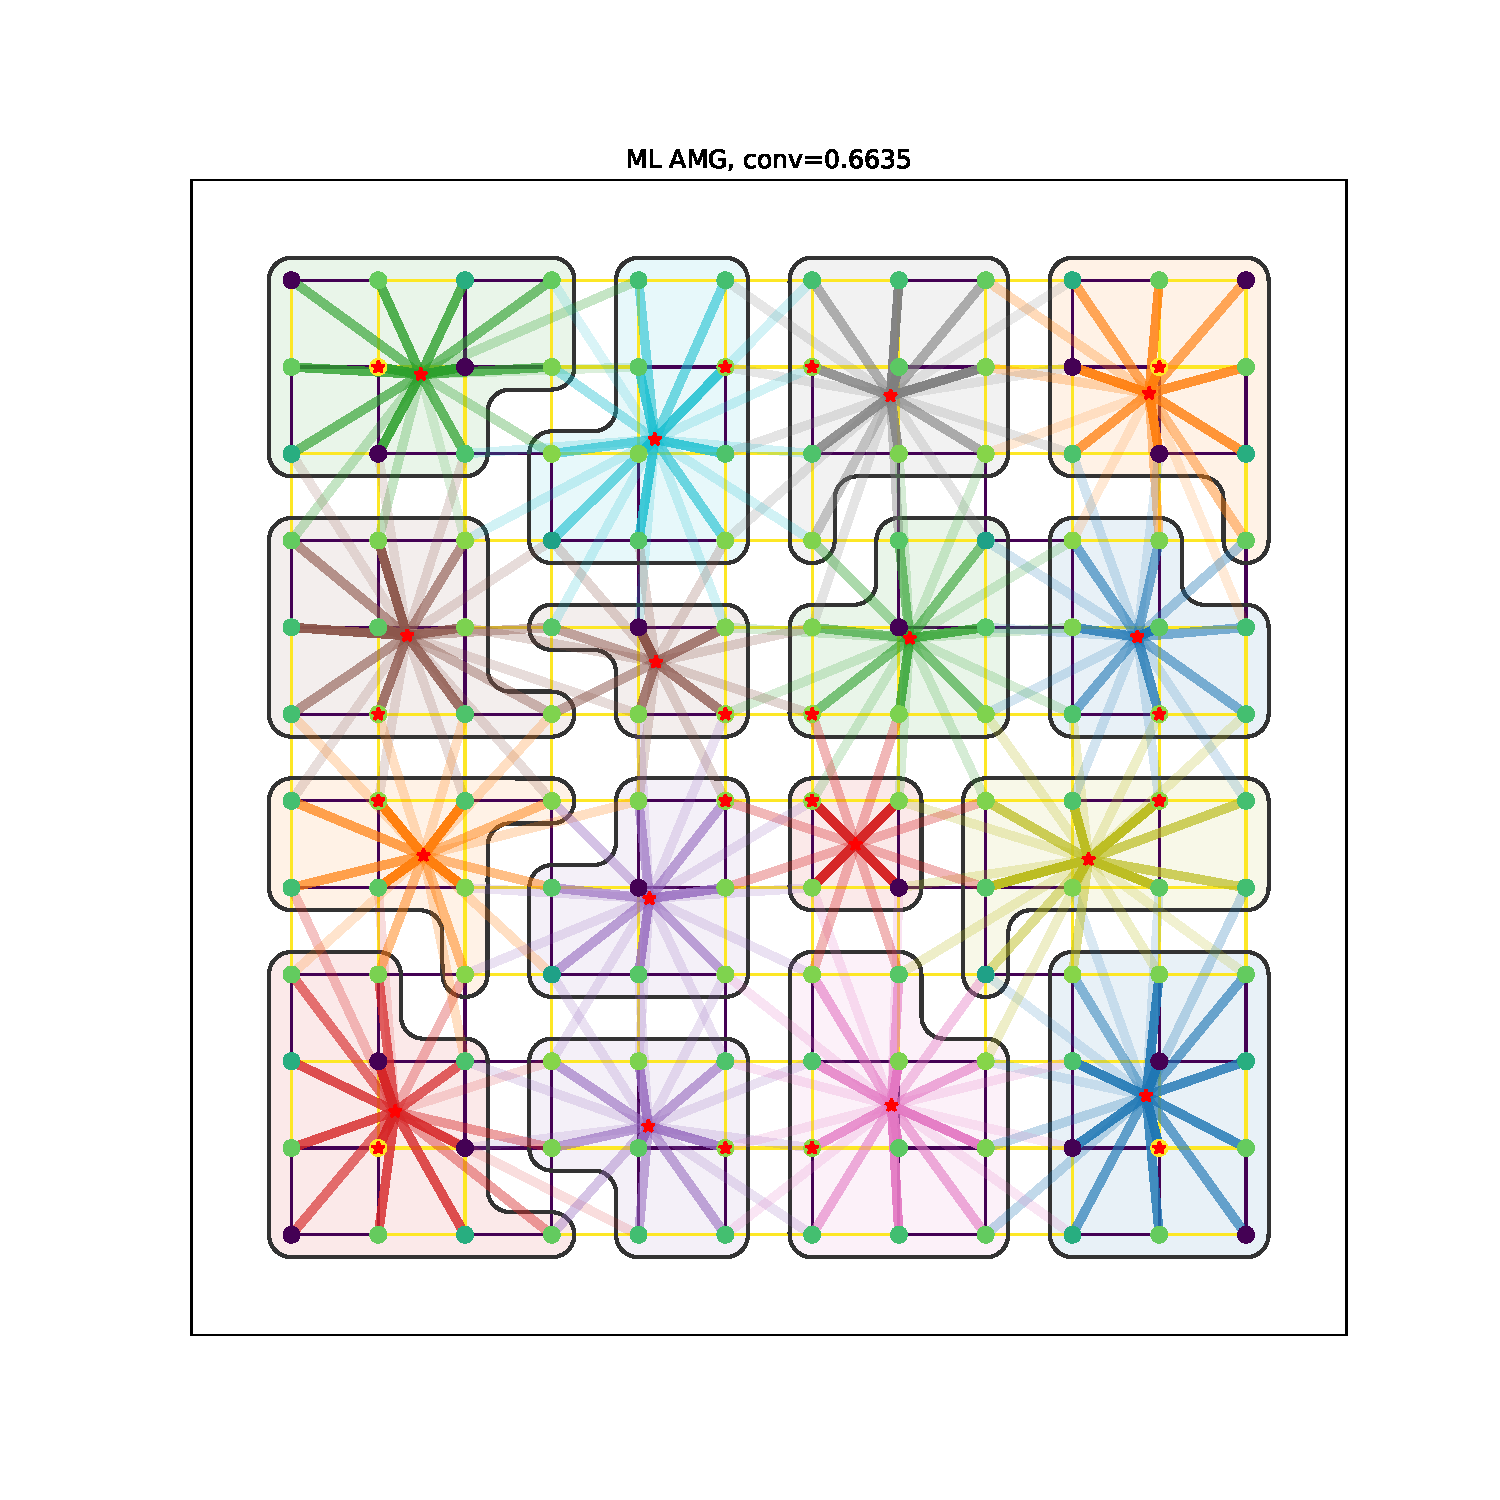
\includegraphics[width=\textwidth]{grid_12_ml.pdf}
    \caption{ML}
  \end{subfigure}
  \caption{Aggregate and interpolation data for a $12 \times 12$ structured grid.}
  \label{fig:grid12}
\end{figure}
\begin{figure}[h]
  \centering
  \begin{subfigure}[t]{0.49\textwidth}
    \centering
    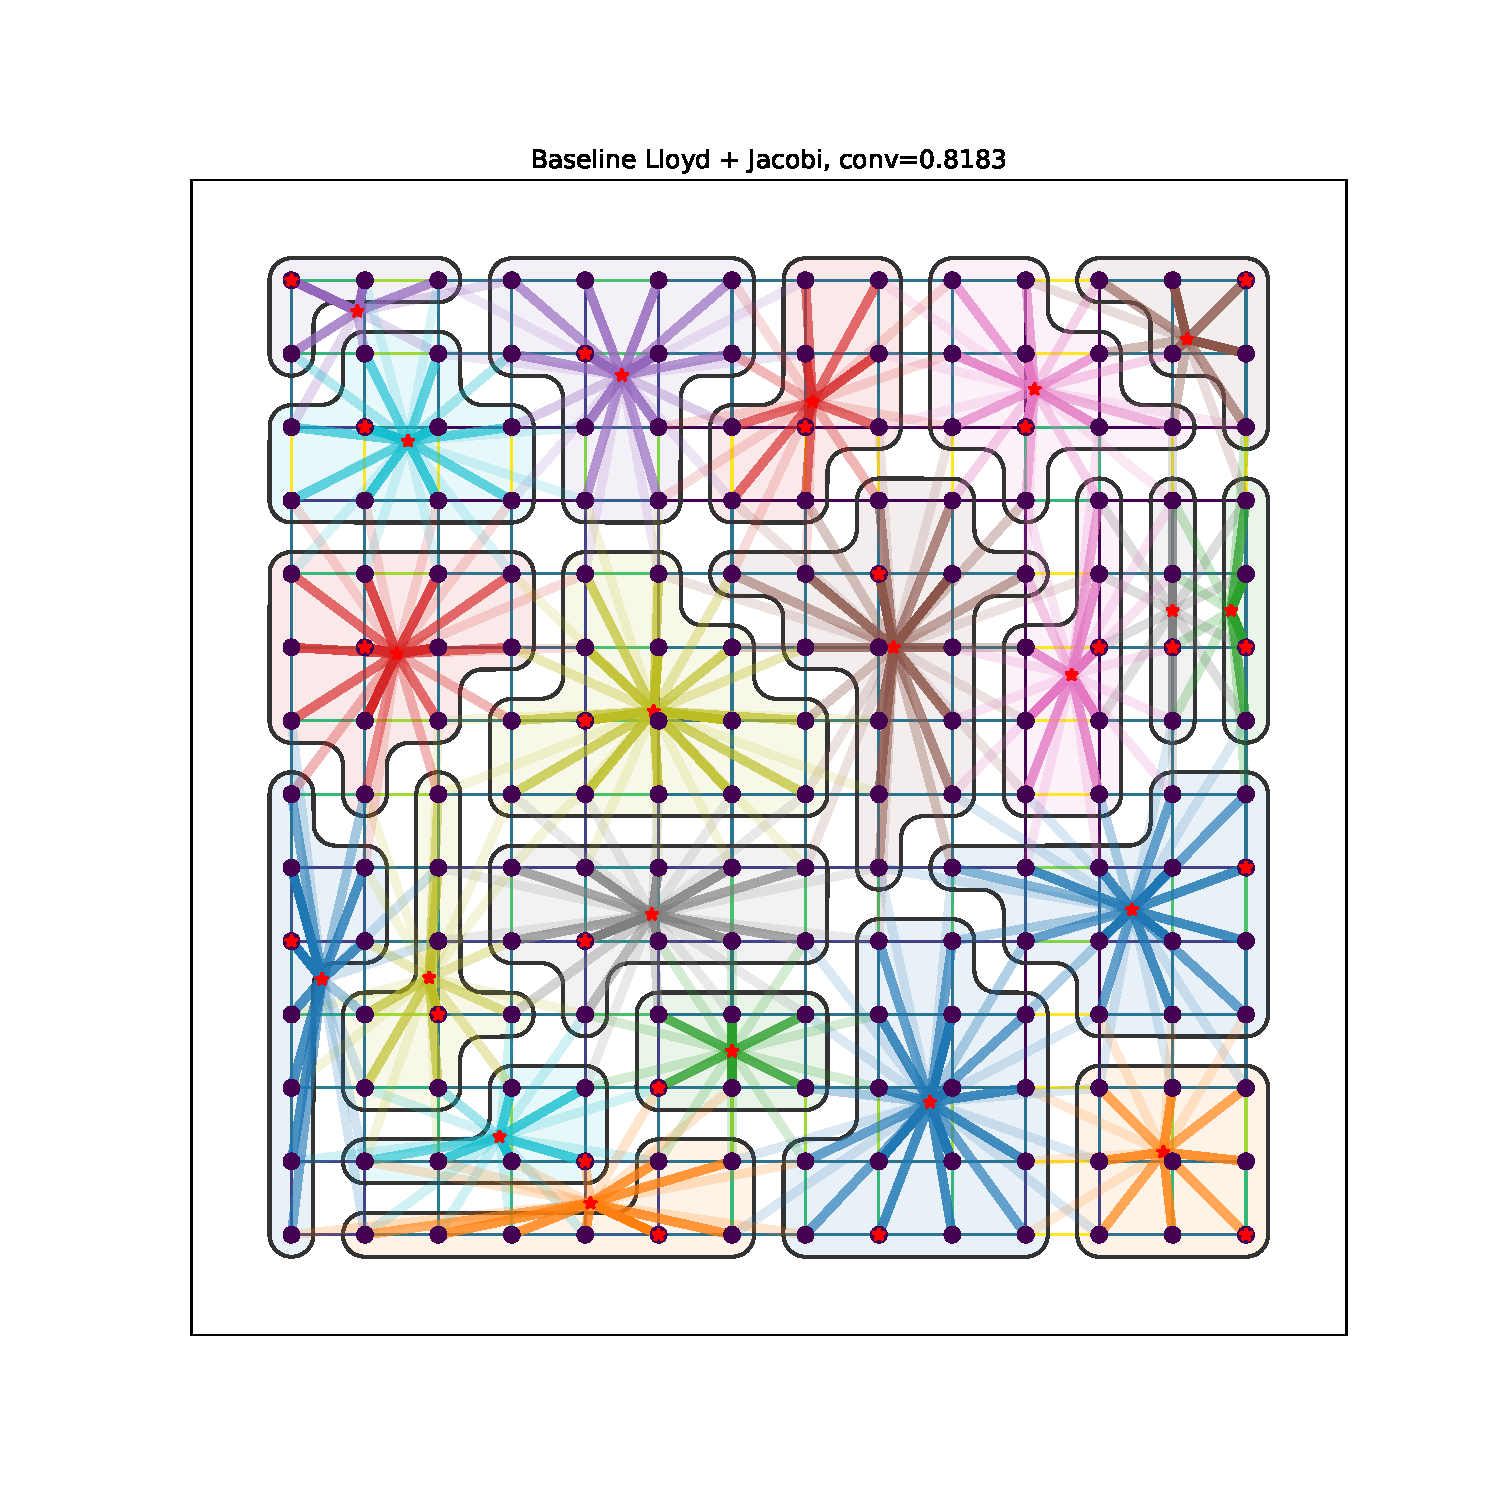
\includegraphics[width=\textwidth]{grid_14_lloyd.pdf}
    \caption{Lloyd + Jacobi}
  \end{subfigure}
  \begin{subfigure}[t]{0.49\textwidth}
    \centering
    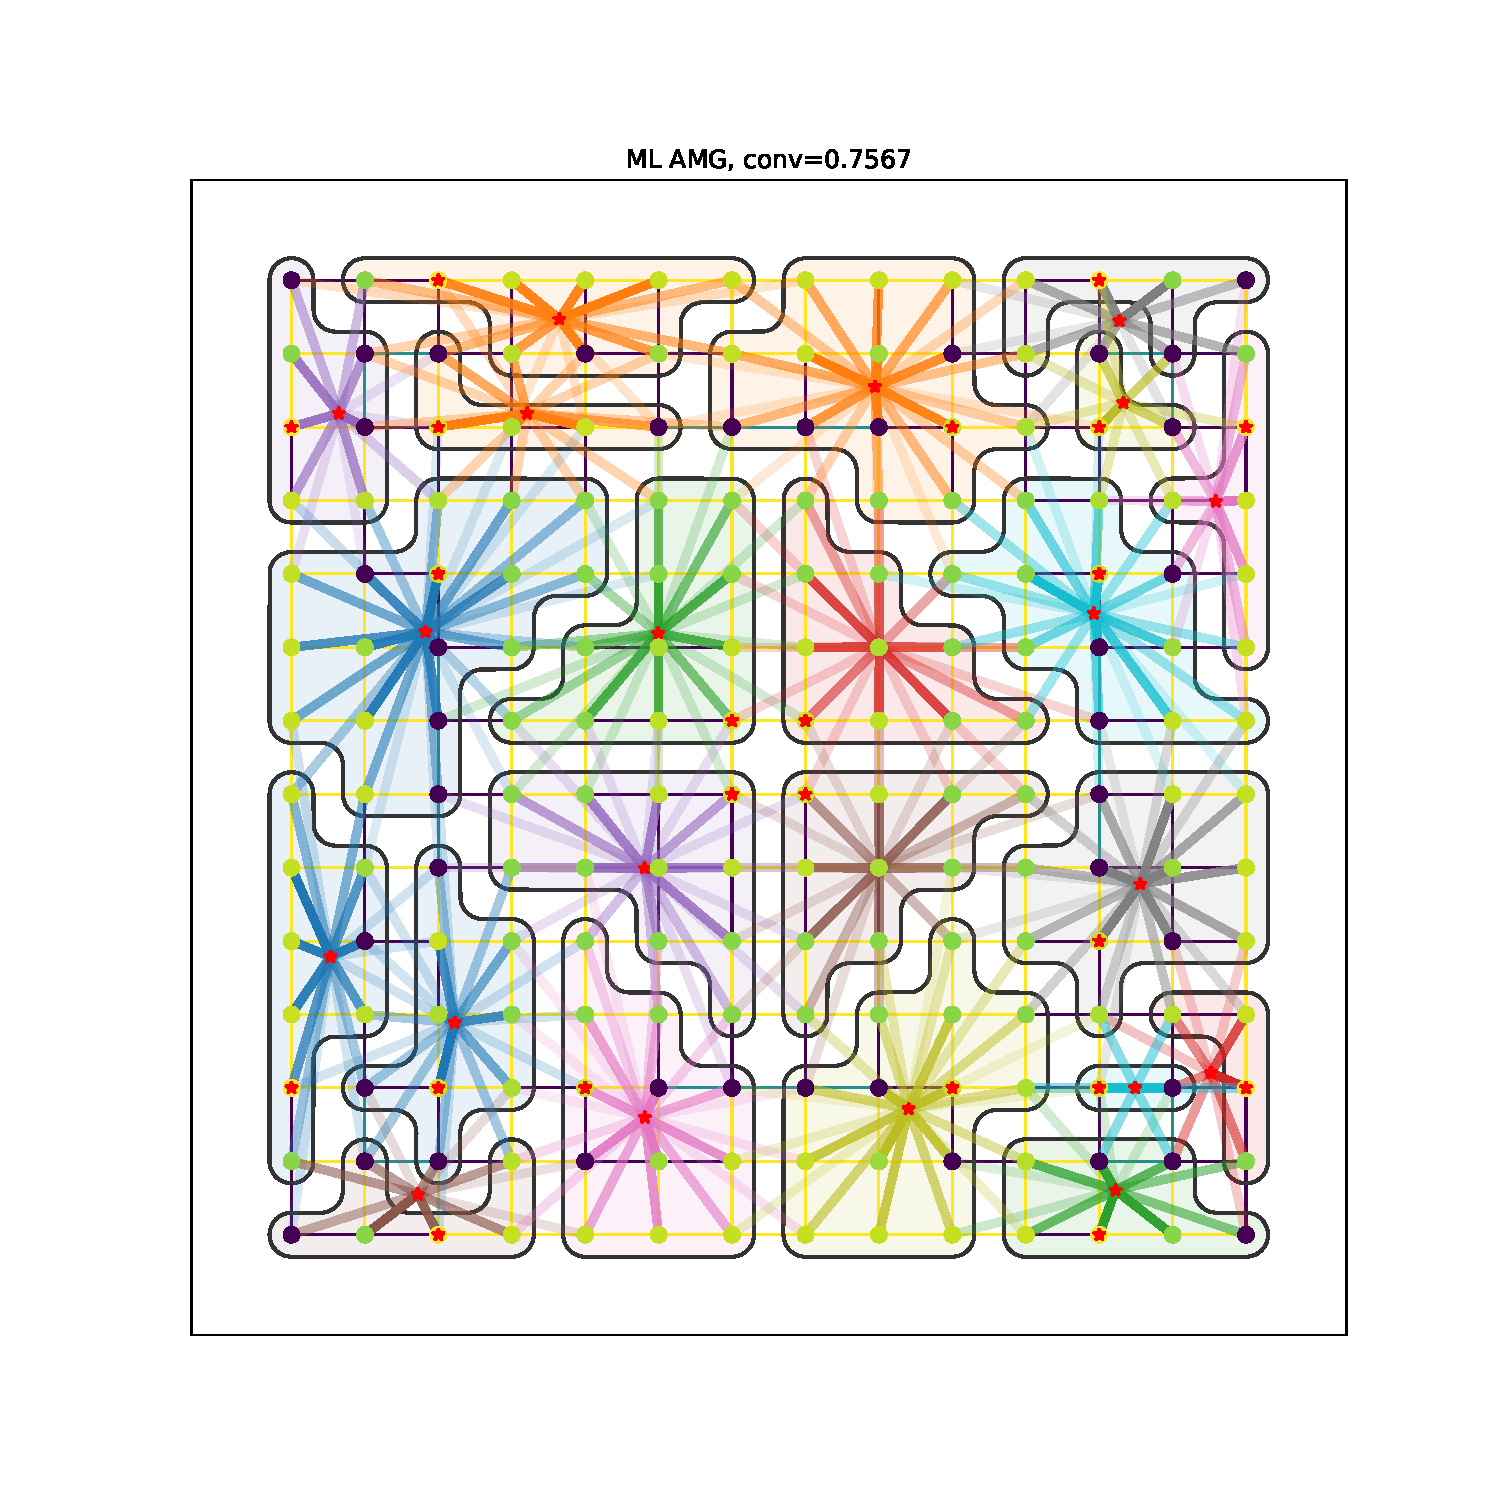
\includegraphics[width=\textwidth]{grid_14_ml.pdf}
    \caption{ML}
  \end{subfigure}
  \caption{Aggregate and interpolation data for a $14 \times 14$ structured grid.}
  \label{fig:grid14}
\end{figure}
\begin{figure}[h]
  \centering
  \begin{subfigure}[t]{0.49\textwidth}
    \centering
    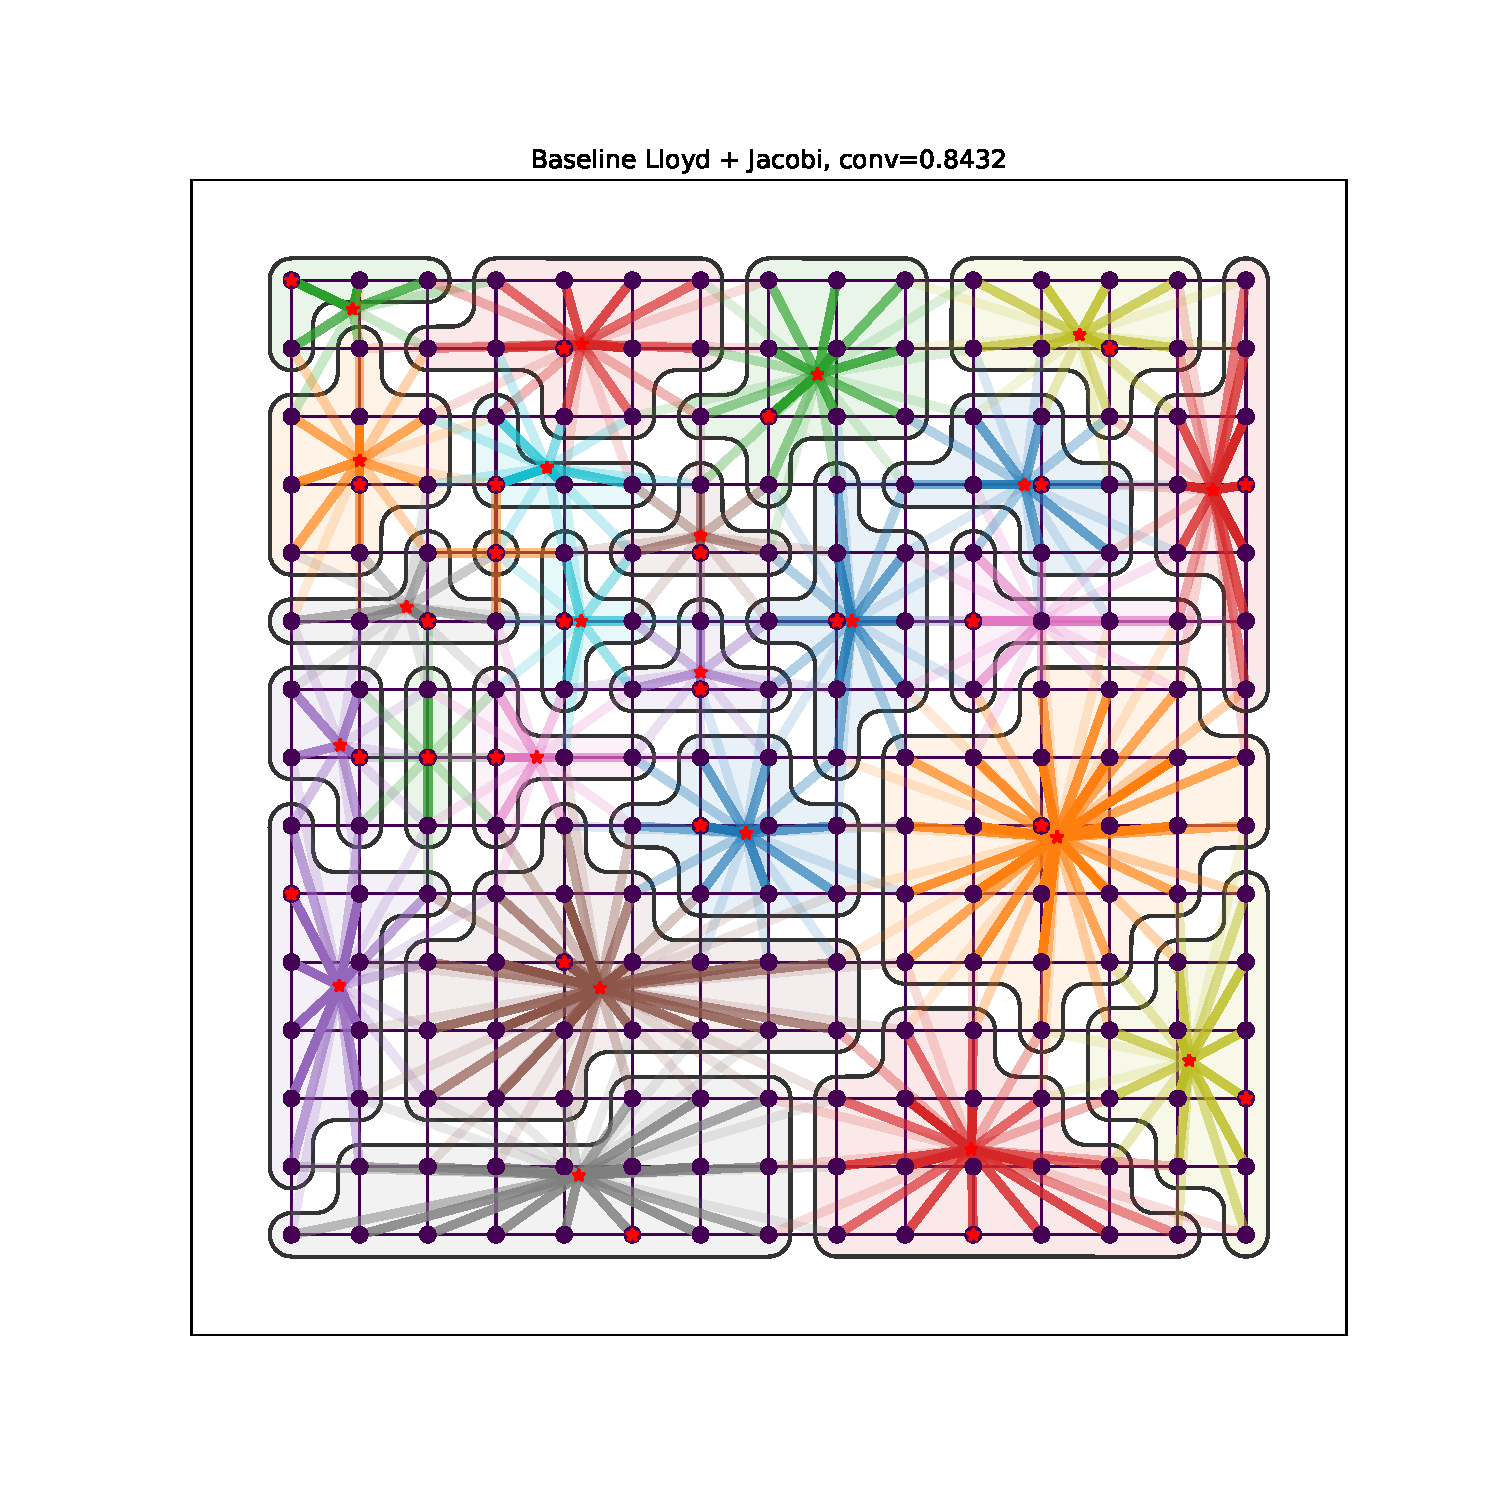
\includegraphics[width=\textwidth]{grid_15_lloyd.pdf}
    \caption{Lloyd + Jacobi}
  \end{subfigure}
  \begin{subfigure}[t]{0.49\textwidth}
    \centering
    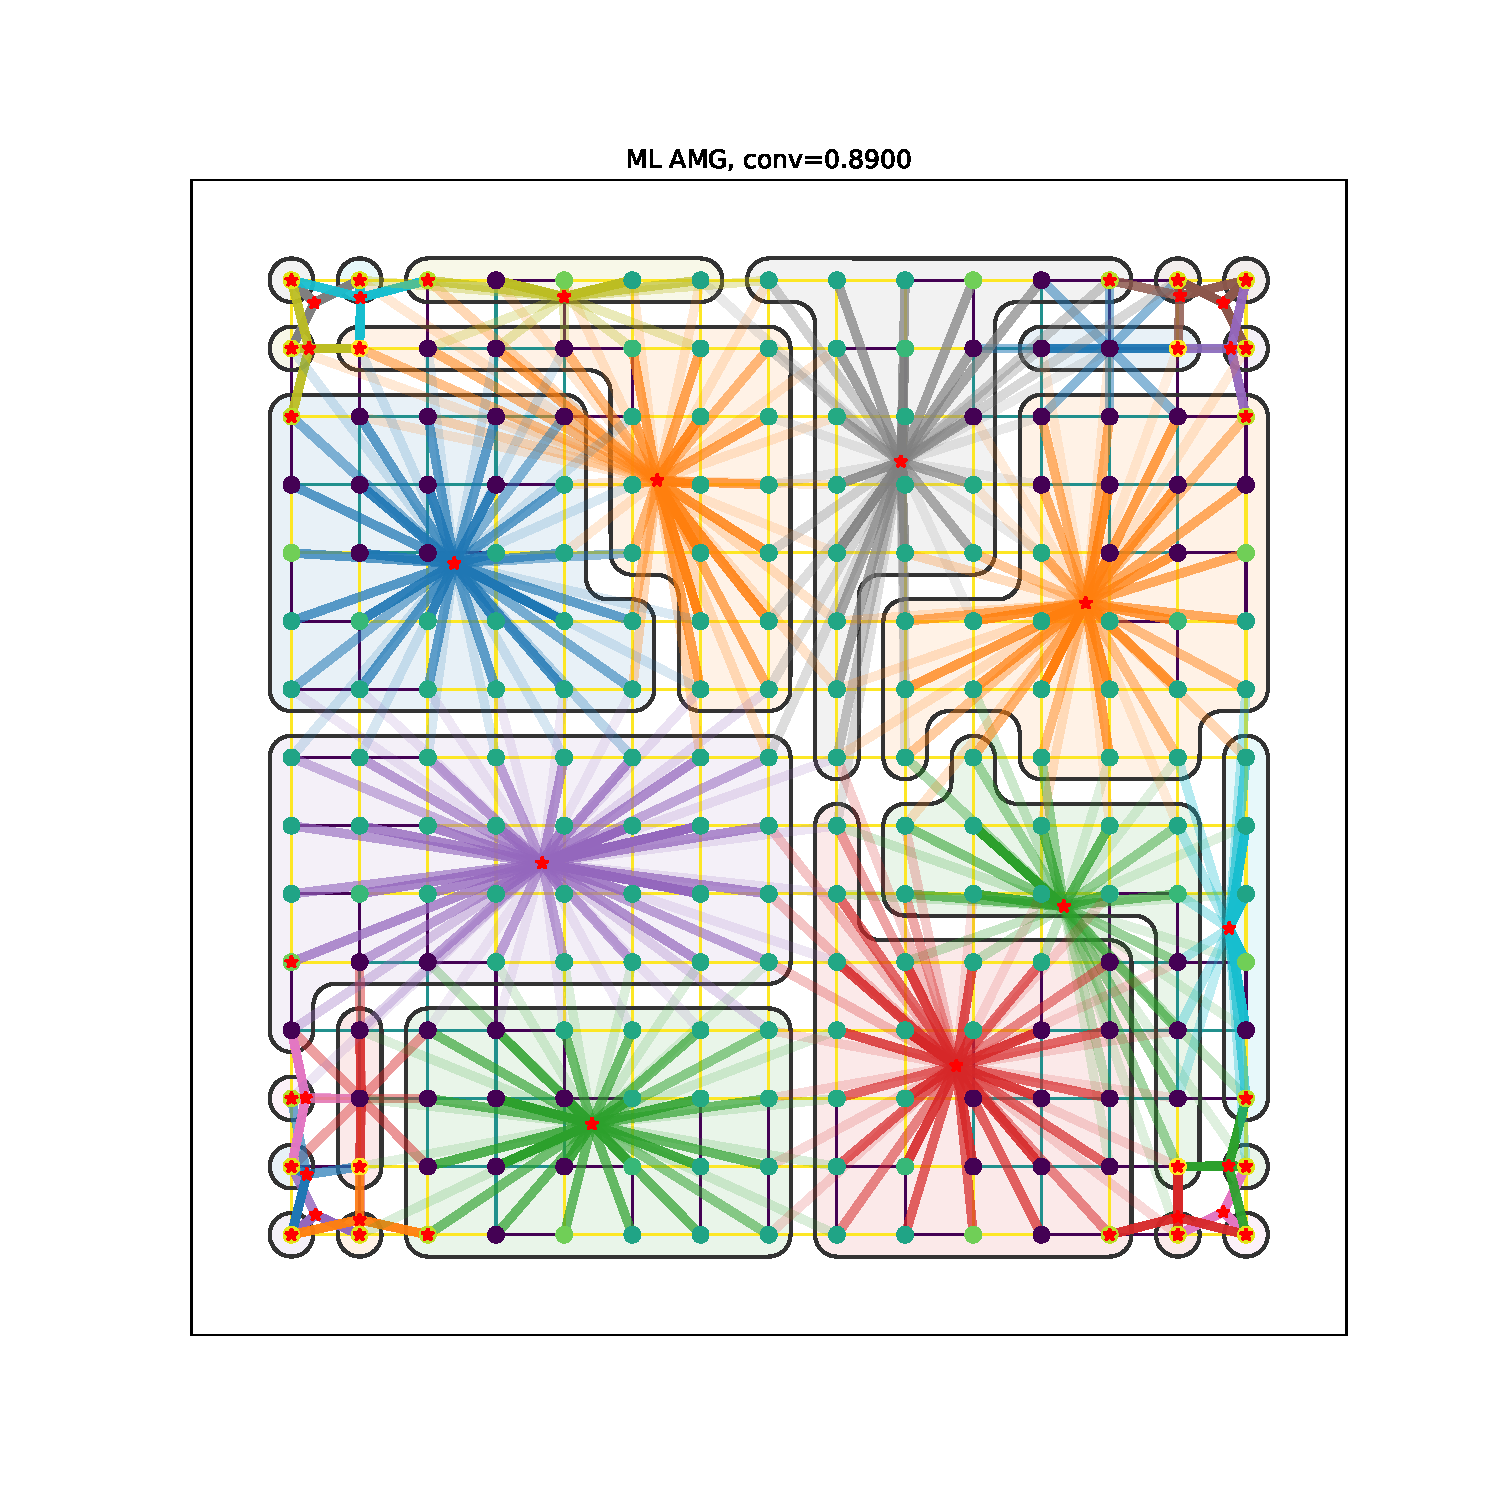
\includegraphics[width=\textwidth]{grid_15_ml.pdf}
    \caption{ML}
  \end{subfigure}
  \caption{Aggregate and interpolation data for a $15 \times 15$ structured grid.}
  \label{fig:grid15}
\end{figure}

Finally, the method is run on an unstructured, circular mesh (Fig \ref{fig:gridcircle}).  The ML method should not have seen anything like this during training, so it is somewhat encouraging that it was able to output a nice set of aggregates.
\begin{figure}[h]
  \centering
  \begin{subfigure}[t]{0.49\textwidth}
    \centering
    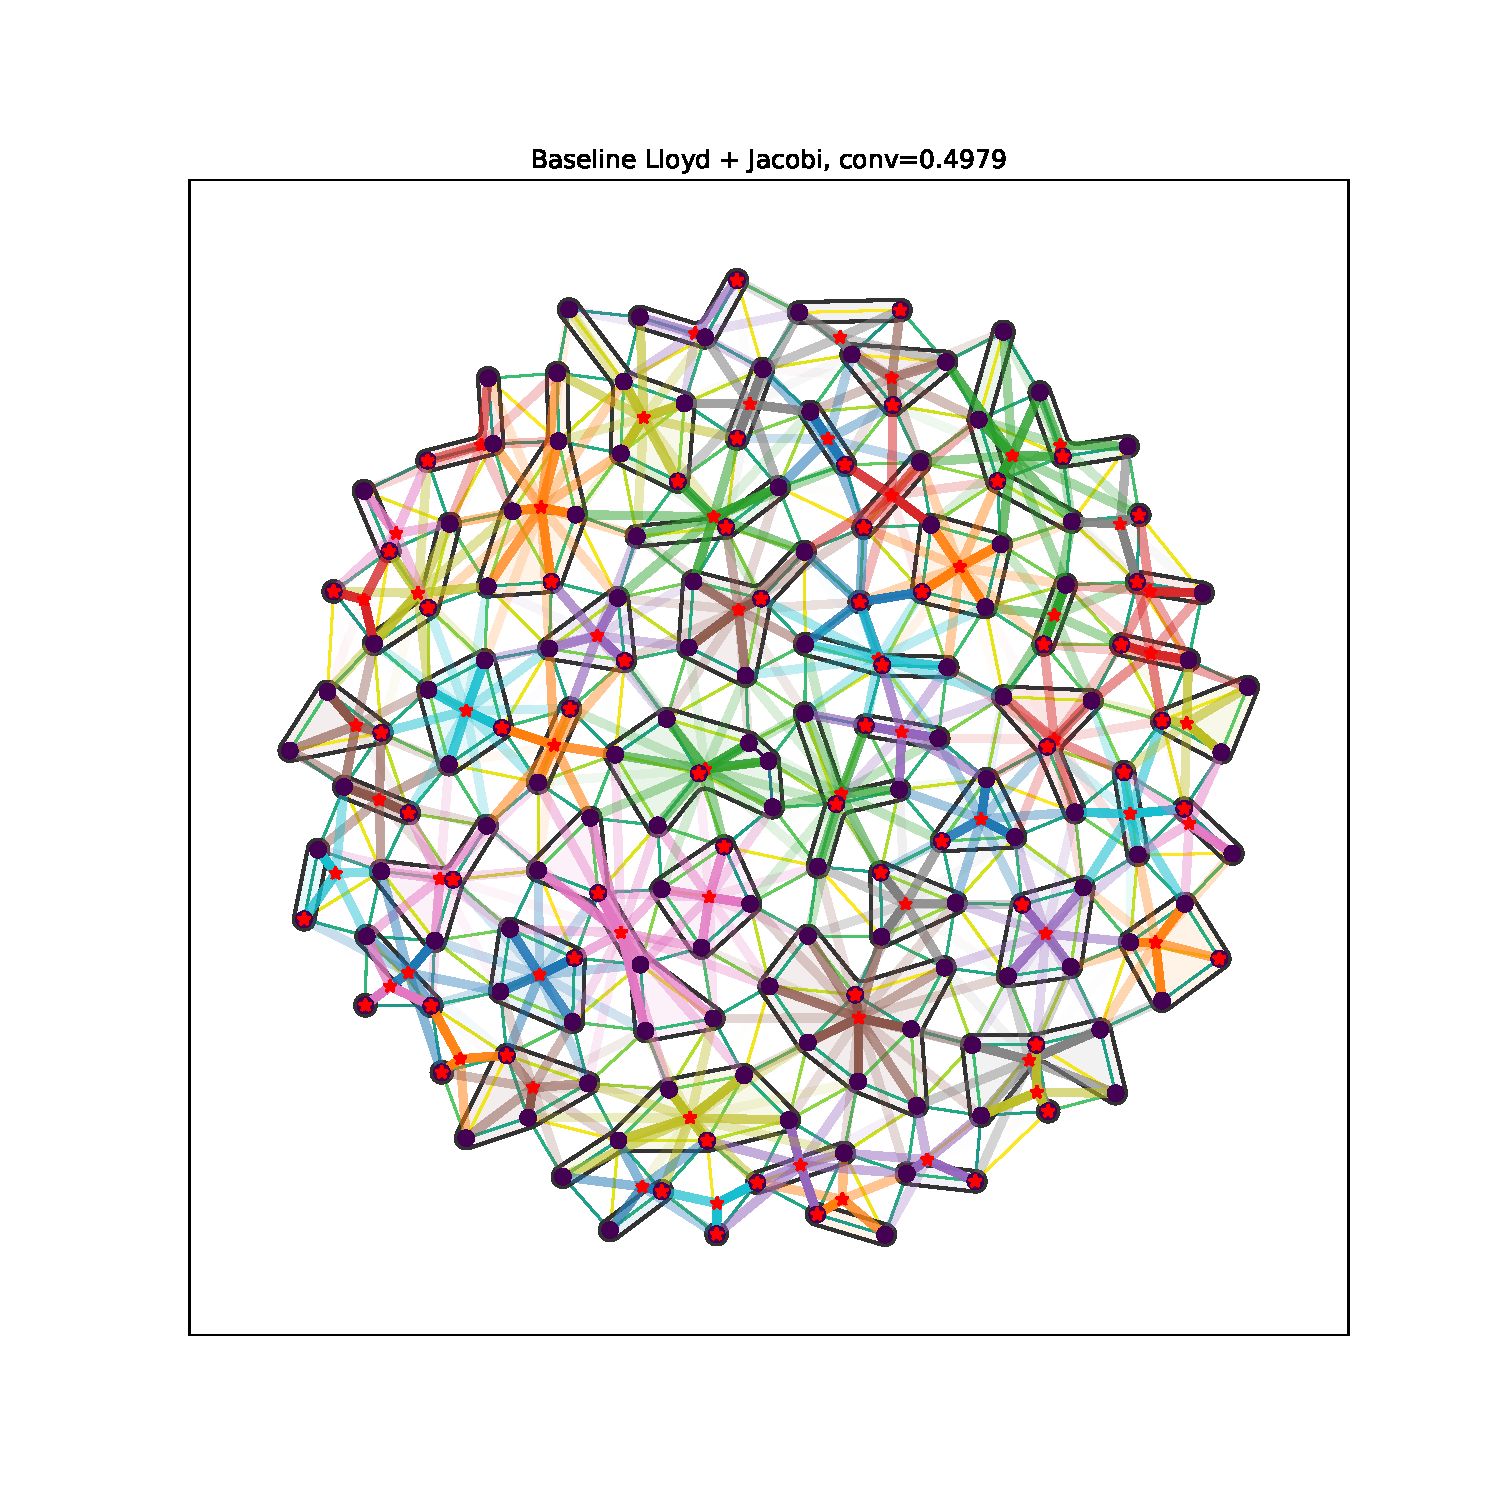
\includegraphics[width=\textwidth]{grid_circle_lloyd.pdf}
    \caption{Lloyd + Jacobi}
  \end{subfigure}
  \begin{subfigure}[t]{0.49\textwidth}
    \centering
    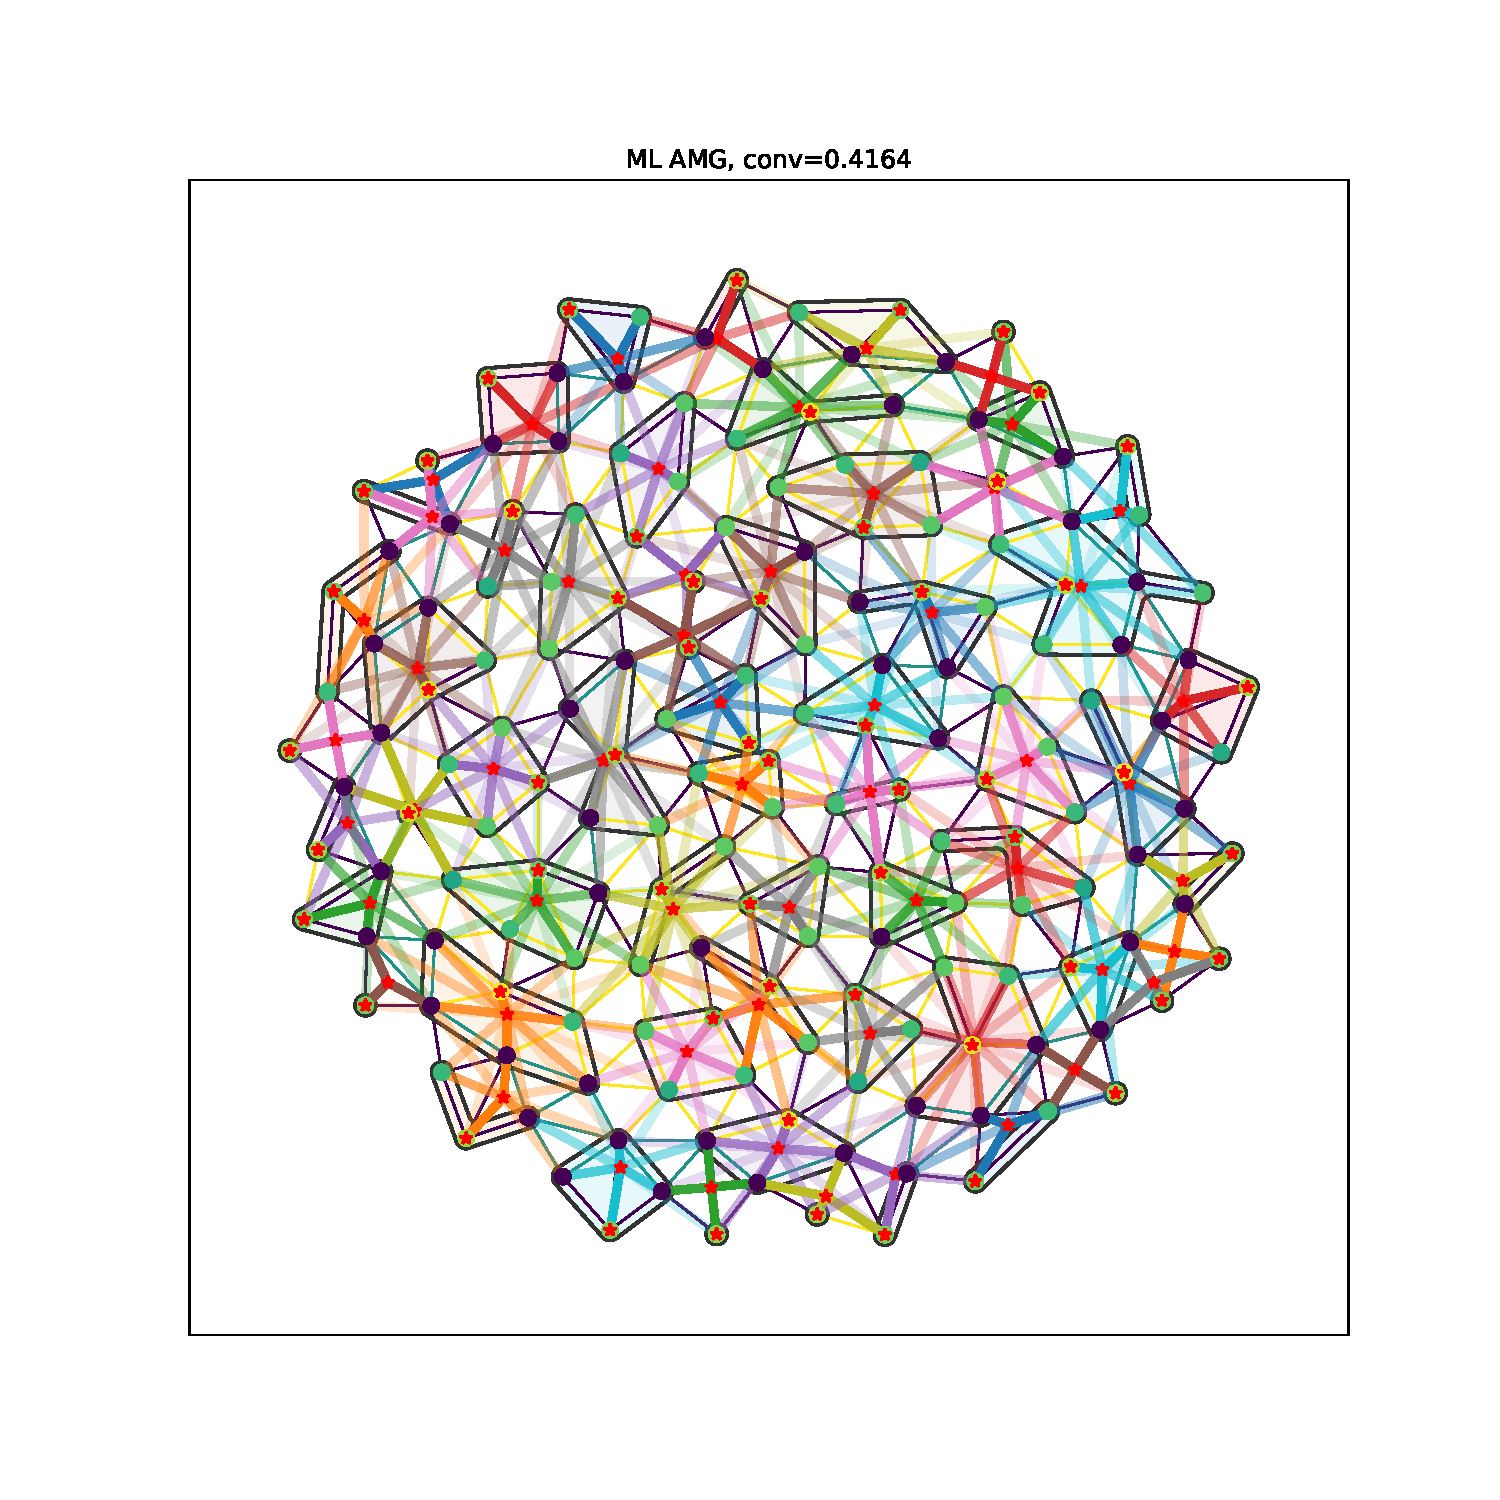
\includegraphics[width=\textwidth]{grid_circle_ml.pdf}
    \caption{ML}
  \end{subfigure}
  \caption{Aggregate and interpolation data for a circular unstructured mesh.}
  \label{fig:gridcircle}
\end{figure}

\section{Future}
The actual training of the ML agent is horribly slow, taking about 13-14 hours just to reach 200 training generations.  If we wanted to train on large datasets, this should probably be addressed.  There are a few things to poke around with:
\begin{enumerate}
\item Fork the PyGAD library (or write our own GA package) and run the fitness calculation in parallel.  This should be \textit{embarassingly parallel}, as we are just doing some large number of AMG iterations to compute convergence.
\item Work out some continuous form of the agent, so we can use a gradient-based optimizer like Adam.  Perhaps there are some tricks to be used to get this working?
\end{enumerate}

\bibliographystyle{siam}
\bibliography{navier}
\end{document}
